\documentclass[11pt,xcolor={svgnames, x11names}]{beamer}
\usefonttheme{professionalfonts}
\usepackage{amsmath}
\usepackage{bm}
\usepackage{graphicx}
\usepackage[many]{tcolorbox}
\usepackage[export]{adjustbox}
% \usepackage{pifont}
% \newcommand{\xmark}{\ding{165}}%

\definecolor{miscstructurecolor}{rgb}{0.65,0.65,0.65}

% \usepackage{enumitem} % incompatible with Beamer?
\everymath{\displaystyle}

\usepackage{tikz}
\usepackage{pgfmath}
\usetikzlibrary{math, calc, intersections, arrows.meta}

% counter for resuming enumerated list numbers
\newcounter{resumeenumi}
\newcommand{\suspend}{\setcounter{resumeenumi}{\theenumi}}
\newcommand{\resume}{\setcounter{enumi}{\theresumeenumi}}

\newcommand\lb{\linebreak}
\newcommand\pars{\par\smallskip}
\newcommand\parm{\par\medskip}
\newcommand\parb{\par\bigskip}

%left flushed minipage
\newcommand{\minit}[2][0.8]{
	\begin{minipage}[t]{#1\columnwidth}
		\raggedright
		#2
	\end{minipage}
}

%left flushed minipage
\newcommand{\mini}[2][0.8]{
	\begin{minipage}[c]{#1\columnwidth}
		\raggedright
		#2
	\end{minipage}
}



% centered minipage with text \raggedright
%\cmini[width]{content}
\newcommand{\cmini}[2][0.8]{
	\begin{center}
		\begin{minipage}{#1\columnwidth}
			\raggedright
			#2
		\end{minipage}
	\end{center}
}

% get x and y coordinates from a tikz coordinate
%\gettikzxy{A}{\ax}{\ay}
\makeatletter
\providecommand{\gettikzxy}[3]{%
	\tikz@scan@one@point\pgfutil@firstofone#1\relax
	\edef#2{\the\pgf@x}%
	\edef#3{\the\pgf@y}%
}
\makeatother

\definecolor{saitMaroon}{RGB}{172, 31, 45}
\definecolor{mucus}{rgb}{0.55,0.53,0.31} 
\definecolor{myGreen}{RGB}{0,150,0}
\definecolor{saitPurple}{RGB}{112,40,119}
\definecolor{saitDeepBlue}{RGB}{0, 99, 167}
\definecolor{saitBlue}{rgb}{0, 0.59, 0.85}


%  \definecolor{saitRed}{RGB}{224,38,37} 

%  \definecolor{khaki}{RGB}{190, 183, 107}
 %\definecolor{philpotBlue}{RGB}{13,69,120}
% \definecolor{dRed}{rgb}{0.7,0,0}
% \definecolor{blueGrey}{rgb}{0.4,0.48,0.53}
% \definecolor{white}{rgb}{1,1,1}
% \definecolor{dkgreen}{rgb}{0,0.5,0}
% \definecolor{greenyellow}{rgb}{0.9,0.9,0.5}
% \definecolor{flesh}{rgb}{1, 0.95, 0.8}
% \definecolor{wheat}{rgb}{.96, .87, .70}
% \definecolor{oldlace}{rgb}{.992, .96187, .902}
% \definecolor{snow}{rgb}{1, .98, .98}
% \definecolor{ghostwhite}{rgb}{.973, .973, 1}
% \definecolor{cornsilk}{rgb}{1, .973, .863}
% \definecolor{honeydew}{rgb}{.941, 1, .941}
% \definecolor{lavenderdark}{rgb}{.8, .8, .9529411}
% \definecolor{lavender}{rgb}{.902, .902, .980}
% \definecolor{lightblue}{rgb}{.8, .8, .95}
\definecolor{lightgray}{rgb}{.827, .827, .827}
% \definecolor{lightsteelblue}{rgb}{.690, .769, .871}
% \definecolor{lightturquoise}{rgb}{.686, .933, .933}
% \definecolor{darkgreen}{rgb}{.0, .392, .0}
% \definecolor{yellowgreen}{rgb}{.604, .804, .196}
% \definecolor{vlightblue}{rgb}{.88, .85, .95}
% \definecolor{khaki}{rgb}{.741, .718, .42}
% \definecolor{lightkhaki}{rgb}{1, .96, .7}
% \definecolor{almostwhite}{rgb}{1,.95,1}
% \definecolor{facegreen}{rgb}{.45, .5, .2}
% \definecolor{llllBlueGrey}{rgb}{0.8,0.96,1}
% \definecolor{lllBlueGrey}{rgb}{0.69,0.83,0.92}
% \definecolor{llBlueGrey}{rgb}{0.58,0.69,0.76}
% \definecolor{lBlueGrey}{rgb}{0.48,0.58,0.64}
% \definecolor{blueGrey}{rgb}{0.4,0.48,0.53}
% \definecolor{dBlueGrey}{rgb}{0.33,0.4,0.44}
% \definecolor{ddBlueGrey}{rgb}{0.28,0.33,0.37}
% \definecolor{dddBlueGrey}{rgb}{0.23,0.28,0.31}
% \definecolor{almostBlue}{rgb}{0.985,0.985,1}
% \definecolor{almostGreen}{rgb}{0.9,0.97,0.9}

% \definecolor{almostRed}{rgb}{0.95,0.875,0.8}
%  \definecolor{headerGrey}{RGB}{128,128,128}
%  \definecolor{headerGray}{RGB}{128,128,128}
% \definecolor{dHeaderGrey}{RGB}{96,96,96}
% \definecolor{ddHeaderGrey}{RGB}{64,64,64}
% \definecolor{dddHeaderGrey}{RGB}{32,32,32}
% \definecolor{lHeaderGrey}{RGB}{160,160,160}
% \definecolor{llHeaderGrey}{RGB}{192,192,192}
% \definecolor{lllHeaderGrey}{RGB}{224,224,224}
% \definecolor{philpotBlue}{RGB}{13,69,120}
% \definecolor{drabGreen}{RGB}{156,143,87}
% \definecolor{ground}{RGB}{153,153,51}
% \definecolor{gridLight}{rgb}{0.85,0.85,0.85}
% \definecolor{darkGreen}{rgb}{0,0.5,0}


\usepackage[absolute,overlay]{textpos}
\setlength{\TPHorizModule}{1.0cm}
\setlength{\TPVertModule}{\TPHorizModule}
\textblockorigin{0.0cm}{0.0cm}  %start all at upper left corner


\usetheme{Antibes}
\usecolortheme[named=miscstructurecolor]{structure}
\setbeamertemplate{items}[triangle]
\setbeamertemplate{blocks}[rounded][shadow=false]
\setbeamertemplate{headline}{\vspace{.1cm}}
\setbeamertemplate{navigation symbols}{} % empty braces suppresses all navigation symbols
\setbeamertemplate{footline}{
	\hfill
	\insertshorttitle
	\quad
	\insertsection
	\quad
	\insertsubsection
	\quad
	\insertframenumber/\inserttotalframenumber
	\quad{ }
	\vspace{0.125cm}
}
\addtobeamertemplate{footline}{\hypersetup{linkcolor=black}}{}
\setbeamertemplate{navigation symbols}{} % empty braces suppresses all navigation symbols
\setbeamercolor{frametitle}{fg=black}

\usepackage{hyperref} % hyperref usually loaded last but automatically by Beamer
\hypersetup{
	colorlinks,
	citecolor=red,
	filecolor=orange,
	bookmarksopen=true,
	linkcolor=staticsstructurecolor, % table of contents
	urlcolor=blue
}
\usepackage{bookmark}

% various hacks to get around (apparent?) Beamer titlepage constraints
\title[\color{black}QWIZM]{\bf\color{black}\Huge QWIZM\normalsize\lb}
\subtitle{Digital Media Design Capstone Project 
in Partial Fulfillment of the Requirements 
for a 
Master of Liberal Arts Degree
} % i.e., a blank line
\institute{\large Dave Morgan}
\author{\LARGE Harvard University Extension School} % another blanky
\date{\small \today}


\everymath{\displaystyle}

\begin{document}
\small
\begin{frame}[plain]
	\titlepage
\end{frame}

%%%%%%%%%%%%%%%%%%%%%%%%%%%%%%%%%%%%%%%%%%%%%%%%%%%%%%%%%%%%%%%%%%%%%%%%%%%%%%%%%%%%%%%%%%%%%%%%%%%%%%%%%%%%%%%%%%%%%%%%
\begin{frame}{\bf Context}

	% \setbeamercolor{normal text}{fg=gray,bg=}
	% % for highlighting current enumeration item
	% \setbeamercolor{alerted text}{fg=black,bg=}
	% \usebeamercolor{normal text}

	\cmini{
		\begin{itemize}
			\item Teaching introductory engineering courses \lb to adults in a two-year Civil Engineering Technology program at a Canadian polytechnic.
			\item Students progress through their program in cohorts of 32 students, each cohort taking the same classes at the same time. Students have about 30 hours of instruction or labs each week. Groups within each cohort become tight-knit and study together.
		\end{itemize}		
	}
\end{frame}	

\begin{frame}{\bf The Problem}

	% \setbeamercolor{normal text}{fg=gray,bg=}
	% % for highlighting current enumeration item
	% \setbeamercolor{alerted text}{fg=black,bg=}
	% \usebeamercolor{normal text}

	\cmini{
		\begin{itemize}
			\item The setting of pertinent take-home assignments that both encourage learning and are efficient to mark.
			\item Exercise solutions tend to be long and complex, involving many steps, and with a reliance on the mathematical accuracy of numerical answers.
			\item Some solutions may involve as many as 40 separate calculations before reaching the final answer.
		\end{itemize}		
	}
\end{frame}	

\begin{frame}{\bf Solutions?}

	\setbeamercolor{normal text}{fg=gray,bg=}
	% for highlighting current enumeration item
	\setbeamercolor{alerted text}{fg=black,bg=}
	\usebeamercolor{normal text}

	\begin{textblock*}{0.95\textwidth}(1cm, 1.55cm)
		\begin{enumerate}			
			\item<1-| alert@1-> A traditional approach: Assigning work from exercises in the course textbook. 
			\item[]<2-> \textcolor{myGreen}{Pros}:
			\begin{itemize}
				\item<2-| alert@2> Convenient to assign or prepare. \textcolor{myGreen}{\large $\bm \checkmark$}
			\end{itemize}
			\item[]<3-> \textcolor{saitMaroon}{Cons}:
			\begin{itemize}				
				\item<3-| alert@3> All students answer the same problems with the same input values, encouraging collaboration. There is a tendency for the strongest student in a group to solve the problem and for the rest to 'understand' the solution without the learning experience of how to develop solutions from basic principles.  \textcolor{saitMaroon}{\large $\bm \times $}  \parm
				\item<4| alert@4> Additionally, students have online access to all major textbook solution manuals making, for many, assignments more a matter of diligent copying than learning. \textcolor{saitMaroon}{\large $\bm \times $}
			\end{itemize}
			% \suspend
		\end{enumerate}		
	\end{textblock*}
\end{frame}	

\begin{frame}{\bf Solutions?}

	\setbeamercolor{normal text}{fg=gray,bg=}
	% for highlighting current enumeration item
	\setbeamercolor{alerted text}{fg=black,bg=}
	\usebeamercolor{normal text}

	\begin{textblock*}{0.9\textwidth}(1cm, 1.55cm)	
		\begin{enumerate}	
			\setcounter{enumi}{1}		
			\item<1-| alert@1-> Using your institution's learning management system (LMS) of choice. These generally offer quizzing/assignment tools with a question type that provides individualized inputs for each student.
		\end{enumerate}
	\end{textblock*}
	\only<2-4>{
		\begin{textblock*}{0.95\textwidth}(1cm, 3.45cm)	
			\begin{itemize}			
				\item[]<2-3| alert@2> Each student gets the same question but with individualized question inputs; they can collaborate on method but have to perform their own calculations.
				\item[]<3| alert@3> Various LMSs offerings: 
					\begin{itemize}
						\item<3| alert@3> Moodle has the `Calculated' question type: \scriptsize\url{https://docs.moodle.org/38/en/Calculated_question_type}
						\item<3| alert@3> Canvas has the `Formula' question type: \scriptsize\url{https://community.canvaslms.com/docs/DOC-26355}
						\item<3| alert@3> Blackboard has the `Calculated Formula' question type: \scriptsize\url{https://help.blackboard.com/Learn/Instructor/Tests_Pools_Surveys/Question_Types/Calculated_Formula_Questions}
					\end{itemize} 
			\end{itemize}
		\end{textblock*}
	}
	\only<4>{
		\begin{textblock*}{0.95\textwidth}(1cm, 3.4cm)	
			\begin{itemize}	
				\item[]<4> \textcolor{myGreen}{Pros}:
				\begin{itemize}
					\item<4| alert@4> Individualized inputs, students perform their own calculations. \textcolor{myGreen}{\large $\bm \checkmark$} \parm
					\item<4| alert@4> Automatic marking of assignments reduces the instructors' workload. \textcolor{myGreen}{\large $\bm \checkmark$}
				\end{itemize}
			\end{itemize}
		\end{textblock*}
	}
	\only<5>{
		\begin{textblock*}{1\textwidth}(1cm, 3.4cm)	
			\begin{itemize}
				\item[]<5> \textcolor{saitMaroon}{Cons}:
				\begin{itemize}
					\item<5| alert@5> Students need to perform many calculations, with no feedback, before submitting their final answer. This often leads to significant student frustration if the question is marked incorrect. \textcolor{saitMaroon}{\large $\bm  \times $} 
					\item<5| alert@5> Instructors do not see students' written work and cannot give feedback on professionalism. \textcolor{saitMaroon}{\large $\bm  \times $}
					\item<5| alert@5> These LMS calculated/formula question types match each student's response to a single formula specified when the question was created. It is not practical to combine a series of up to 40 calculations into a single equation. \textcolor{saitMaroon}{\large $\bm  \times $}
					\item<5| alert@5> Many problems require more than a single answer. \lb E.g., finding the three angles of a triangle. \textcolor{saitMaroon}{\large $\bm  \times $}
				\end{itemize}			
			\end{itemize}
		\end{textblock*}
	}	
	
\end{frame}	


\begin{frame}{\bf Solutions?}

	\setbeamercolor{normal text}{fg=gray,bg=}
	% for highlighting current enumeration item
	\setbeamercolor{alerted text}{fg=black,bg=}
	\usebeamercolor{normal text}

	\only<2-3>{
		\begin{textblock*}{0.425\textwidth}(7cm, 1.75cm)	
			\cfig[0.25]{./images/moodleQuiz.png}
		\end{textblock*}
	}
	\only<4->{
		\begin{textblock*}{0.425\textwidth}(8.9cm, 1cm)	
			\cfig[0.12]{./images/moodleQuiz.png}
		\end{textblock*}
	}
	\begin{textblock*}{0.75\textwidth}(1cm, 1.55cm)	
		\begin{enumerate}	
			\setcounter{enumi}{2}		
			\item<1-| alert@1-> {\bfseries If} your institution uses Moodle, and {\bfseries if} you are able persuade your system administrator to install a specific plug-in, the `Formulas' type plug-in allows multiple question parts. \scriptsize\url{https://moodle.org/plugins/qtype_formulas}
		\end{enumerate}
	\end{textblock*}
	\only<2-3>{
	\begin{textblock*}{0.5\textwidth}(1cm, 3.85cm)	
		\begin{itemize}				
			\item[]<2-|alert@2> A typical statics question using the `Formulas' plug-in, as shown here, has 10 input fields for the results of separate calculations.
			\item[]<3-> \textcolor{myGreen}{Pros}:
			\begin{itemize}
				\item<3| alert@3> If you have access to Moodle and the `Formulas' plug-in, this may be a good route to follow. \textcolor{myGreen}{\large $\bm \checkmark$} \parm				
			\end{itemize} 
		\end{itemize}
	\end{textblock*}
	}
	\only<4->{
		\begin{textblock*}{0.95\textwidth}(1cm, 3.85cm)	
			\begin{itemize}
				\item[] \textcolor{saitMaroon}{Cons}:
					\begin{itemize}
						\item<4| alert@4> Access limited to Moodle platform users. \textcolor{saitMaroon}{\large $\bm  \times $} 
						\item<4| alert@4> Plug-ins, not part of the Moodle core, may break when Moodle is updated. \textcolor{saitMaroon}{\large $\bm  \times $}
						\item<4| alert@4> Moodle is open source and plug-ins are maintained by volunteers. Due to retirement, there is no current maintainer of the `Formula' plug-in. \textcolor{saitMaroon}{\large $\bm  \times $}
						\item<4|alert@4> 	`Instant' feedback for each part has to be `gamed': After each answer is entered, you must submit the whole question for marking and then look for a checkmark indicating your last entry is correct. \textcolor{saitMaroon}{\large $\bm  \times $}
					\end{itemize} 
			\end{itemize}
		\end{textblock*}
	}	
\end{frame}	

\begin{frame}{\bf Enter Qwizm!}
	\begin{itemize}
		\item \url{qwizm.org} is an existing web-site containing containing an early proof-of-concept for this current version of Qwizm. Although limited in content, it has proved useful for over ten years and is still in use by former colleagues.
		\item The existing site will be replaced by the new application as questions are converted to the new format.
		\item All the code from the original app has been refactored. Features that are new to this current version are indicated. 
		% \item Quizzes are comprised of an arbitrary number of questions, each question comprised of an arbitrary number of parts.
		% \item Questions requiring multiple answers are suitable for step-by-step progression through a typically complex take-home or in-class assessment problem set commonly found in introductory engineering technology courses.
		% \item Instant marking of each submission is provided by an `Enter' button adjacent to each answer input field.
	\end{itemize}

\end{frame}	

\begin{frame}
	\centering
	\setlength{\fboxsep}{0pt}%
	\setlength{\fboxrule}{0.5pt}%
	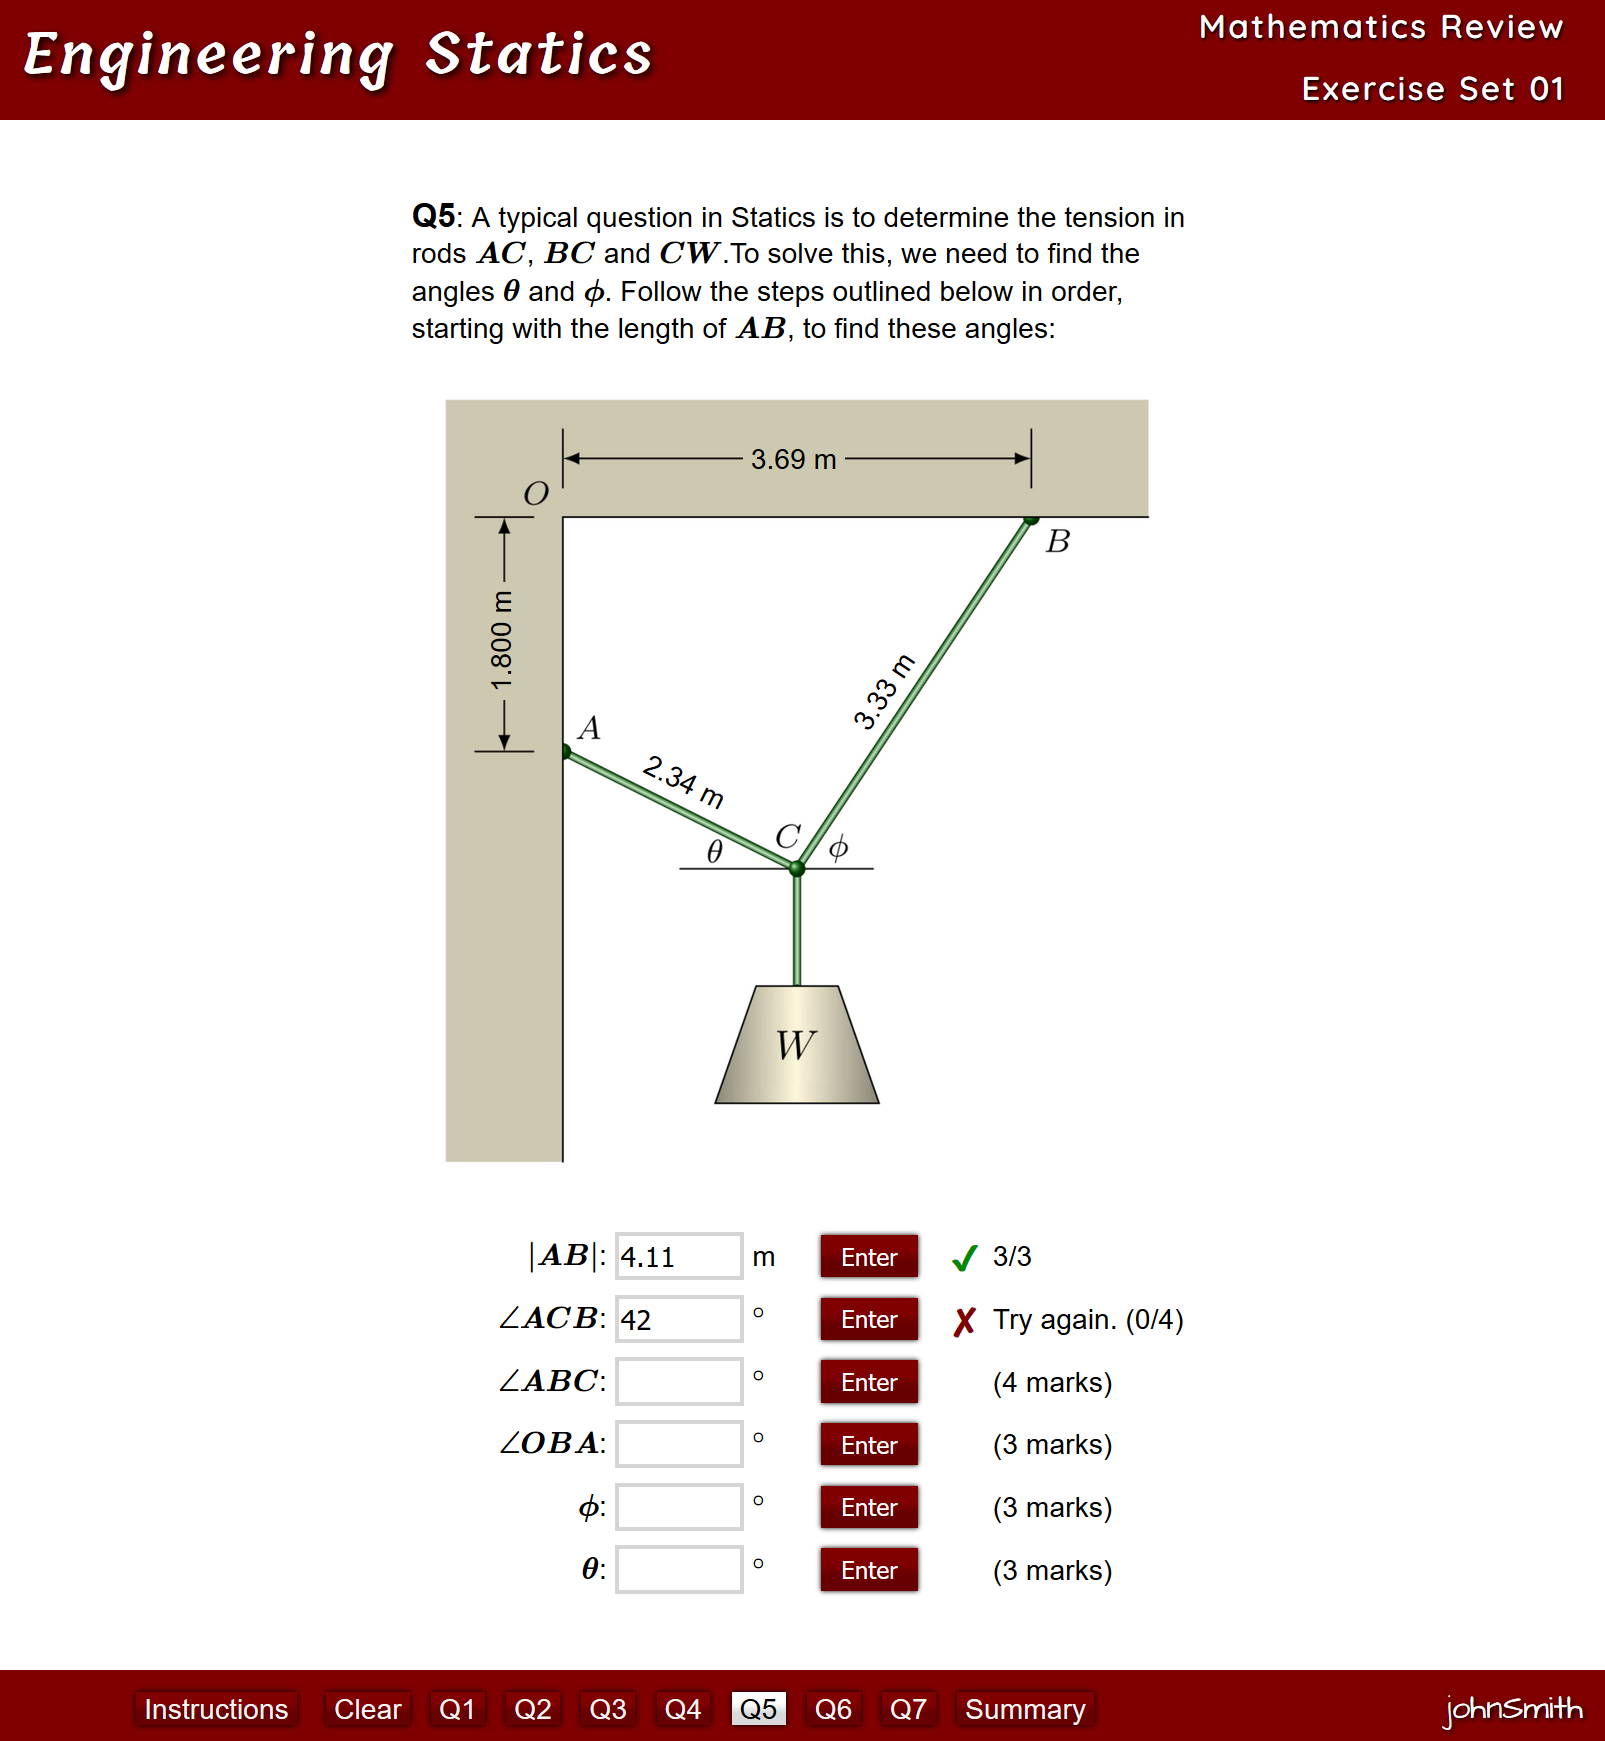
\includegraphics[scale=0.29, cfbox=gray]{./images/cover.png}	
\end{frame}	

% \begin{frame}{\bf Qwizm}
% 	\begin{itemize}
% 		\item \url{qwizm.org} is an existing web-site containing containing an early proof-of-concept for this current version of Qwizm. Although limited in content, it has proved useful for over ten years and is still in use by former colleagues.	
% 		\item All the code from the original app has been refactored. Features that are new to this current version are indicated.	
% 	\end{itemize}
% \end{frame}

\begin{frame}{\bf Qwizm}
 
	\begin{itemize}	
		\item<1->[] \textcolor{myGreen}{\bf Pros}:
		\begin{itemize}	[<+->] 	
			\item Quizzes are comprised of an arbitrary number of questions. \textcolor{myGreen}{\large $\bm \checkmark$}
			\item Questions are comprised of an arbitrary number of parts. \textcolor{myGreen}{\large $\bm \checkmark$}
			\item Instant marking of each submission is provided by an `Enter' button adjacent to each answer input field. \textcolor{myGreen}{\large $\bm \checkmark$}
			\item \textcolor{myGreen}{New!} Using \texttt{localStorage}, Qwizm now is able to store user inputs between sessions and return to the view that the user was on when closing the previous session. \textcolor{myGreen}{\large $\bm \checkmark$}
			\item \textcolor{myGreen}{New!} Qwizm is now responsive. \textcolor{myGreen}{\large $\bm \checkmark$} 
			\item \textcolor{myGreen}{New!} Individualized question variables can now be placed over a colored background and/or rotated. \textcolor{myGreen}{\large $\bm \checkmark$}
			\item \textcolor{myGreen}{New!} Able to render math using the math type-setting language \LaTeX{} \textcolor{myGreen}{\large $\bm \checkmark$}
			\item \textcolor{myGreen}{New!} Some limited feedback for incorrect answers. \textcolor{myGreen}{\large $\bm \checkmark$} 
			\item Completely client-side. \textcolor{myGreen}{\large $\bm \checkmark$} 			
		\end{itemize}
		\item<10->[] \textcolor{saitMaroon}{\bf Cons}:
		\begin{itemize}
			\item Completely client-side. \textcolor{saitMaroon}{\large $\bm \times $} 
		\end{itemize}
	\end{itemize}
\end{frame}

\begin{frame}{\bf Client-side?}
 
	\begin{itemize}	
		\item<1->[] \textcolor{myGreen}{\bf Pros}:
		\begin{itemize}	[<+->] 	
			\item No need to manage user data on the server. (I'm not looking for a long term commitment here, just the ability to add quizzes and questions when the urge strikes.) \textcolor{myGreen}{\large $\bm \checkmark$}	
		\end{itemize}
		\item<1->[] \textcolor{saitMaroon}{\bf Cons}:
		\begin{itemize}
			\item No automatic entry of student marks or attempts to an LMS gradebook. \textcolor{saitMaroon}{\large $\bm \times $} 
			\begin{itemize}
				\item This is less of a problem for instructors than might first seem obvious. There is more paper handling, of course, with a summary printout and written work attached but marking is very quick. It is the work of a moment to scan the written work for professionalism and that some (or all) work matches the submitted answers. Then, assign to mark to the student in the gradebook. It takes about a minute to `mark' a student Qwizm assignment. And, commonly, you are marking long complex problems. 
			\end{itemize}
		\end{itemize}
	\end{itemize}
\end{frame}

\begin{frame}{\bf Client-side?}
 
	\begin{itemize}			
		\item<1->[] \textcolor{saitMaroon}{\bf Cons}:
		\begin{itemize}	
		
		\item Nothing's secret in the browser; the user can find anything! \textcolor{saitMaroon}{\large $\bm \times $}\parm \pause
			\begin{enumerate} [<+->]				
				\item[] True enough, but:	\parm			
				\item In ten years of using the proof-of-concept original version of Qwizm, this never happened. \pars
				\item Work is in progress on a masking function for answers accessible in the browser. (Should be done by the end of the week...)\pars
				\item Even with the correct answer located, students have to come up with the written work to arrive at that number. \pars
				\item Each assignment is worth about 1\% of the final course work so there is not a lot at stake. \pars The stated purpose is assessment but, in reality, it's more about guided learning, encouraging a student through a long problem towards a final answer. It is formative assessment rather than summative assessment.
					
			\end{enumerate} 
		\end{itemize}
	\end{itemize}
\end{frame}

\begin{frame}{Technologies Used}
	\begin{itemize}
	 	\item The core of the application is HTML5, CSS3 and ES6 (Javascript)
	 	\item jQuery is used to facilitate DOM manipulation and reduce browser compatibility issues.
	 	\item The katex ({\small\url{https://katex.org/}}) javascipt library is used for math typesetting in the \LaTeX language
	 	\item The ES6 is compiled into ES5 so that current browsers can read it. Babel ({\small\url{https://babeljs.io/}}) is run to perform the compilation.
	 	\item VSCode is the editor used for development. I made regular use of its live server.
	 	\item CSS styles were automatically compiled when SASS files were saved using the Live Sass Compiler extension for VSCode.
		\item All development was on a Windows 10 laptop. 
		\item Code is open source and available at {\small\url{https://github.com/dmorgorg/nuQwizm}}
	 	
	\end{itemize}
\end{frame}

% \begin{frame}{Suggested Use-Case}
% 	lskdjf
% \end{frame}

% \begin{frame}{Overlay Feature}
% 	lskdjf
% \end{frame}

\begin{frame}{Going Live!}
	Let's see it in action: \lb
	\url{https://qwizm.org/nuQwizm/statics/quizzes/quiz00MR01/}
\end{frame}



\begin{frame}{\bf Why not host the app within an LMS?}
	\begin{itemize}
		\item It is not simple, or even possible in many cases, to insert a functioning .html site containing JavaScript into an LMS. 
		\begin{itemize}
			\item The LMS with which I have most experience, D2L Brightspace, automatically strips all JavaScript to the extent that it is not possible to include simple JavaScript libraries in pages. Other LMSs may do the same.\pars
			\item There is a plug-in ({\scriptsize\url{https://github.com/ricoshae/ricoshaejs}}) for inserting `JavaScript activities' into Moodle. The LMS interface for entering code into Moodle -- without the intellisense, syntax highlighting and live browser updating available in modern text-editors -- complicates content creation and makes debugging difficult.
		\end{itemize}
		\item Having a relatively lightweight application, hosted on a openly available site, ensures free access for all who are interested.
		
	\end{itemize}

\end{frame}	

\begin{frame}{\bf Future Plans}

	\setbeamercolor{normal text}{fg=gray,bg=}
	% for highlighting current enumeration item
	\setbeamercolor{alerted text}{fg=black,bg=}
	\usebeamercolor{normal text}
	\begin{enumerate}
		
		\item<1-|alert@1> Improve marking options:
		\begin{itemize}
			\item Allow a specified tolerance in the last digit of an answer. \lb E.g., if the correct answer to a question is $1.234$, also allow $1.233$ and $1.235$ as correct answers. This may be useful in the case of questions with many calculations that allow rounding errors to accumulate. \pars
			\item Allow the option of a certain percentage of error in the answer.
		\end{itemize}\parm
		\item<2-|alert@2> Introduce the concept of `question sets'. Currently, each student gets the same question but with individualized inputs. With questions sets, two or more questions of equal difficulty and testing equivalent concepts may be chosen at random for display in the quiz. In this case, not all students get the same questions; their question is chosen `randomly' from an array of equivalent questions.
	\end{enumerate}

\end{frame}	

\begin{frame}{\bf Future Plans}

	\setbeamercolor{normal text}{fg=gray,bg=}
	% for highlighting current enumeration item
	\setbeamercolor{alerted text}{fg=black,bg=}
	\usebeamercolor{normal text}
	\begin{enumerate}
		\setcounter{enumi}{2}
		\item<1-|alert@1> Masking of correct solutions:
		\begin{itemize}
			\item A user who knows their way around their browser's debugger can readily find `correctSoln' in a stored variable.\footnote[frame,1]{In more than 10 years using a prototype of Qwizm, I was never aware of any of my students finding correct answers in this way. Given the tight-knit nature of my student cohorts, I feel that if one student knew how to do this then all would soon know. The queries I received from students having difficulties getting thie correct answers indicated that they were unaware of the debuggers capabilities.} \pars
			\item Encoding and decoding functions are under development (not quite ready yet!). 
			Instead of `correctSoln' containing $1.234$, it will contain something like `VM\`{}VDCG.EA9'. \scriptsize\url{https://codepen.io/dmorgorg/pen/dyPJbLQ}
		\end{itemize}
	\end{enumerate}

\end{frame}	

\begin{frame}{\bf Future Plans}

	\setbeamercolor{normal text}{fg=gray,bg=}
	% for highlighting current enumeration item
	\setbeamercolor{alerted text}{fg=black,bg=}
	\usebeamercolor{normal text}
	\begin{enumerate}
		\setcounter{enumi}{3}
		\item<1-|alert@1-> Creation of an quiz and question authoring tool:
	\end{enumerate}
	\begin{itemize}
		\item<2-|alert@2> Although outside the scope of this capstone project, this proposed authoring tool (Qwizard) is my primary motivation for this refactoring of Qwizm. \pars
		\item<3-|alert@3> A frequent refrain from colleagues has been that Qwizm is only useful for the courses that I have created content for. They cannot develop quizzes and questions for the courses that they teach without learning to program JavaScript.\pars
		\item<4-|alert@4> This current version of Qwizm has been developed with an authoring tool in mind. When complete, Qwizard will allow an instructor without specific programming knowledge to develop questions that can be saved to their desktop. Instructors will be able to create their own library of questions. Quizzes will be made from a selection of already created questions. A quiz can then be exported to a single .html file which can be either hosted or emailed directly to students. \pars
		\item<5-|alert@5> Qwizard will be written in HTML, CSS and JavaScript and will use Electron to convert it into a desktop application.
	\end{itemize}
\end{frame}

\begin{frame}{The Elevator Pitch!}
	~
\end{frame}

% \begin{frame}[plain]
% 	\begin{textblock*}{0.95\textwidth}(5cm, 5cm)
% 		\HUGE QWIZM!
% 	\end{textblock*}
% \end{frame}

	

\end{document}
